% ============================================================
%  IEEE Pipeline Diagram — Spatial Intelligence System
%  Compile with:  pdflatex pipeline_diagram.tex
%
%  Layout (left → right):
%   Video Input → Frame Extraction →[COLMAP → NeRF]→[YOLO+SAM → Ray Proj]→ 3D Scene Graph → LLM Agent
%   where [...] denotes labelled group boxes
% ============================================================

\documentclass[tikz, border=6pt]{standalone}
\usepackage{tikz}
\usetikzlibrary{
  shapes.geometric,
  arrows.meta,
  positioning,
  fit,
  backgrounds
}

\begin{document}
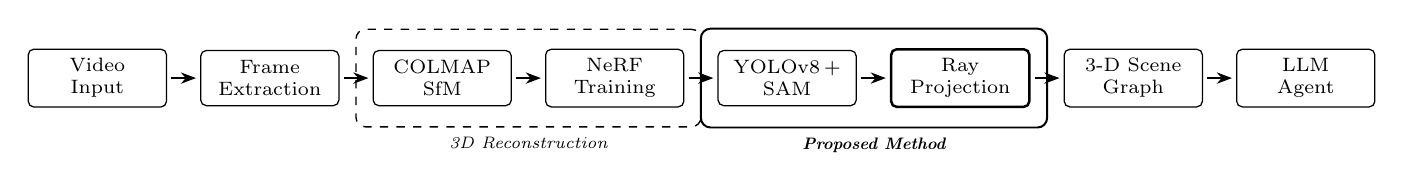
\begin{tikzpicture}[
  % ── Base block ──────────────────────────────────────────
  block/.style={
    rectangle,
    rounded corners = 2pt,
    draw            = black,
    line width      = 0.45pt,
    fill            = white,
    text width      = 1.52cm,
    align           = center,
    minimum height  = 0.70cm,
    font            = \fontsize{7}{8}\selectfont
  },
  % ── Highlighted block (core method) ─────────────────────
  coreblock/.style={
    block,
    draw       = black,
    line width = 0.90pt,
  },
  % ── Arrow ───────────────────────────────────────────────
  arr/.style={
    -Stealth,
    line width  = 0.55pt,
    shorten >=  1.5pt,
    shorten <=  1.5pt
  },
  % ── Group-box label ─────────────────────────────────────
  grplbl/.style={
    font   = \fontsize{6.5}{7}\selectfont\itshape,
    anchor = north
  }
]

% ── Nodes ──────────────────────────────────────────────────
\node[block]                        (vid)  {Video\\Input};
\node[block, right=0.42cm of vid]   (frm)  {Frame\\Extraction};
\node[block, right=0.42cm of frm]   (col)  {COLMAP\\SfM};
\node[block, right=0.42cm of col]   (nerf) {NeRF\\Training};
\node[block, right=0.42cm of nerf]  (yolo) {YOLOv8\,+\\SAM};
\node[coreblock, right=0.42cm of yolo] (ray)  {Ray\\Projection};
\node[block, right=0.42cm of ray]   (sg)   {3-D Scene\\Graph};
\node[block, right=0.42cm of sg]    (llm)  {LLM\\Agent};

% ── Arrows ─────────────────────────────────────────────────
\foreach \f/\t in {vid/frm, frm/col, col/nerf, nerf/yolo,
                   yolo/ray, ray/sg, sg/llm}
  \draw[arr] (\f) -- (\t);

% ── Group 1: 3D Reconstruction (dashed border) ─────────────
\begin{scope}[on background layer]
  \node[
    draw          = black,
    dashed,
    rounded corners = 3.5pt,
    line width    = 0.50pt,
    fill          = white,
    inner xsep    = 6pt,
    inner ysep    = 7pt,
    fit           = (col)(nerf),
    label         = {[grplbl]below:3D Reconstruction}
  ] (grp1) {};
\end{scope}

% ── Group 2: Proposed Method (solid border) ─────────────────
\begin{scope}[on background layer]
  \node[
    draw          = black,
    rounded corners = 3.5pt,
    line width    = 0.72pt,
    fill          = white,
    inner xsep    = 6pt,
    inner ysep    = 7pt,
    fit           = (yolo)(ray),
    label         = {[grplbl]below:\textbf{Proposed Method}}
  ] (grp2) {};
\end{scope}

\end{tikzpicture}
\end{document}
